\begin{figure}[t]
\centering
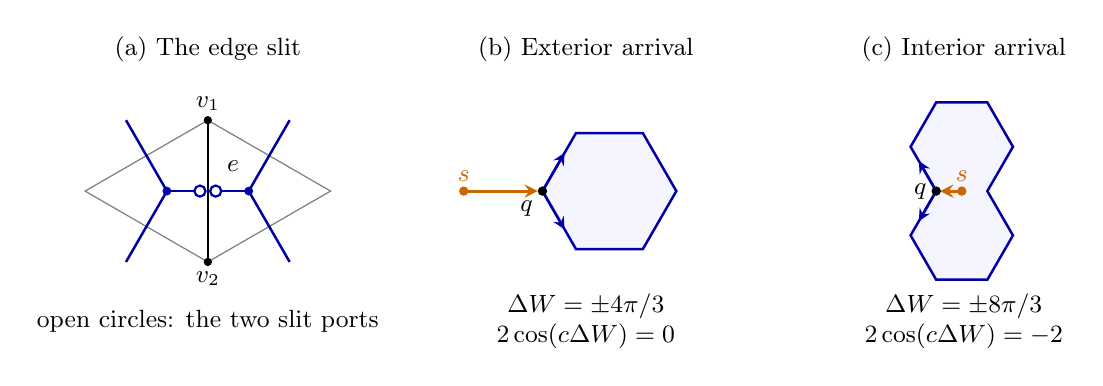
\begin{tikzpicture}[x=1cm,y=1cm,>=stealth,font=\small,
  primal/.style={draw=black!50,line width=.45pt},
  dual/.style={draw=blue!65!black,line width=.9pt},
  arrival/.style={draw=orange!80!black,line width=1.1pt,->}]
\begin{scope}
  \node at (0,1.8) {(a) The edge slit};
  \draw[primal] (0,.9)--(-1.55885,0)--(0,-.9)
                (0,.9)--(1.55885,0)--(0,-.9);
  \draw[black,line width=.7pt] (0,.9)--(0,-.9);
  \draw[dual] (-1.03923,.9)--(-.519615,0)--(-1.03923,-.9)
              (1.03923,.9)--(.519615,0)--(1.03923,-.9);
  \draw[dual] (-.519615,0)--(-.10,0)
              (.10,0)--(.519615,0);
  \fill[blue!65!black] (-.519615,0) circle(1.6pt);
  \fill[blue!65!black] (.519615,0) circle(1.6pt);
  \draw[blue!65!black,fill=white,line width=.8pt]
        (-.10,0) circle(2pt) (.10,0) circle(2pt);
  \fill (0,.9) circle(1.5pt) node[above] {$v_1$};
  \fill (0,-.9) circle(1.5pt) node[below] {$v_2$};
  \node[above right] at (.12,.13) {$e$};
  \node[align=center] at (0,-1.65)
    {open circles: the two slit ports};
\end{scope}
\begin{scope}[xshift=4.8cm]
  \node at (0,1.8) {(b) Exterior arrival};
  \path[fill=blue!4] (-.55,0)--(-.125,.736122)--(.725,.736122)
      --(1.15,0)--(.725,-.736122)--(-.125,-.736122)--cycle;
  \draw[dual] (-.55,0)--(-.125,.736122)--(.725,.736122)
      --(1.15,0)--(.725,-.736122)--(-.125,-.736122)--cycle;
  \draw[dual,->] (-.55,0)--(-.27,.484974);
  \draw[dual,->] (-.55,0)--(-.27,-.484974);
  \draw[arrival] (-1.55,0)--(-.61,0);
  \fill[orange!80!black] (-1.55,0) circle(1.7pt)
      node[above] {$s$};
  \fill (-.55,0) circle(1.7pt) node[below left] {$q$};
  \node[align=center] at (0,-1.65)
    {$\Delta W=\pm4\pi/3$\\$2\cos(c\Delta W)=0$};
\end{scope}
\begin{scope}[xshift=9.6cm]
  \node at (0,1.8) {(c) Interior arrival};
  \path[fill=blue!4] (-.35,0)--(-.675,.562917)--(-.35,1.125834)
      --(.30,1.125834)--(.625,.562917)--(.30,0)
      --(.625,-.562917)--(.30,-1.125834)--(-.35,-1.125834)
      --(-.675,-.562917)--cycle;
  \draw[dual] (-.35,0)--(-.675,.562917)--(-.35,1.125834)
      --(.30,1.125834)--(.625,.562917)--(.30,0)
      --(.625,-.562917)--(.30,-1.125834)--(-.35,-1.125834)
      --(-.675,-.562917)--cycle;
  \draw[dual,->] (-.35,0)--(-.57,.381051);
  \draw[dual,->] (-.35,0)--(-.57,-.381051);
  \draw[arrival] (-.025,0)--(-.30,0);
  \fill[orange!80!black] (-.025,0) circle(1.7pt)
      node[above] {$s$};
  \fill (-.35,0) circle(1.7pt) node[left] {$q$};
  \node[align=center] at (0,-1.65)
    {$\Delta W=\pm8\pi/3$\\$2\cos(c\Delta W)=-2$};
\end{scope}
\end{tikzpicture}
\caption{The slit and the two first-repeat cancellations, with $c=3/8$.
In (a), black and grey segments are primal tiling sides and blue segments
are honeycomb bonds. The bond crossing the side $v_1v_2$ is cut at its
midpoint $e$; the two slit ports are separated slightly for visibility.
Panels (b) and (c) are schematic representatives. The orange leg is
the first prefix arrival at $q$ from the slit source $s$. The path then
traverses the blue cycle and returns to $q$, its first repeated dual
vertex. The two arrows leaving $q$ indicate the two cycle
orientations. Their additional rotations are $\pm4\pi/3$ when $s$ is
outside the cycle and $\pm8\pi/3$ when $s$ is inside. In (c), the arrival
leg occupies the reflex interior sector at $q$.}
\label{fig:slit}
\end{figure}
